%%%%%%%%%%%%%%%%%%%%%%%%%%%%%%%%%%%%%%%%%%%%%%%%%%%%%%%%%%%%%%%%%%%%%%%%%%%%%%%
\documentclass[a4paper,12pt, oneside]{article}

%%%%%%%%%%%%%%%%%%%%%%%%%%%%%%%%%%%%%%%%%%%%%%%%%%%%%%%%%%%%%%%%%%%%%%%%%%%%%%%
\usepackage{tabu}
\usepackage{hhline}
\usepackage{extsizes}
\usepackage{cmap}
\usepackage[T2A]{fontenc}
\usepackage[utf8x]{inputenc}
\usepackage[english, russian]{babel}
\usepackage{misccorr}
\usepackage{amssymb,amsfonts,amsmath,amsthm}  % математические дополнения от АМС
% \usepackage{envmath}  % многострочные формулы EqSystem
\usepackage{indentfirst} % Включение отступа первой строки раздела
\usepackage[usenames,dvipsnames]{color} % названия цветов

%%%%%%%%%%%%%%%%%%%%%%%%%%%%%%%%%%%%%%%%%%%%%%%%%%%%%%%%%%%%%%%%%%%%%%%%%%%%%%%

	% выбрать цвета:
% \definecolor{BlueGreen}{RGB}{49,152,255}

%%%%%%%%%%%%%%%%%%%%%%%%%%%%%%%%%%%%%%%%%%%%%%%%%%%%%%%%%%%%%%%%%%%%%%%%%%%%%%%

	% назначить цвета при подключении hyperref
\usepackage[unicode, colorlinks, urlcolor=magenta, linkcolor=black, pagecolor=black]{hyperref}
	% linkcolor=
	% цвет гиперссылок внутри документа, по-умолчанию red
	% pagecolor=
	% цвет гиперссылок на другие страницы внутри документа, по-умолчанию red
	% filecolor=
	% цвет гиперссылок, открывающих локальные файлы, по-умолчанию cyan
	% anchorcolor=
	% цвет текста мишени, по-умолчанию black
	% citecolor=
	% цвет библиографических ссылок, по-умолчанию green
	% urlcolor=
	% цвет гиперссылок на сетевые ресурсы, по-умолчанию magenta

%%%%%%%%%%%%%%%%%%%%%%%%%%%%%%%%%%%%%%%%%%%%%%%%%%%%%%%%%%%%%%%%%%%%%%%%%%%%%%%

	% улучшенное форматирование таблиц
\usepackage{makecell} 
\usepackage{multirow} 

%%%%%%%%%%%%%%%%%%%%%%%%%%%%%%%%%%%%%%%%%%%%%%%%%%%%%%%%%%%%%%%%%%%%%%%%%%%%%%%

	% подчеркивания
\usepackage{ulem}

%%%%%%%%%%%%%%%%%%%%%%%%%%%%%%%%%%%%%%%%%%%%%%%%%%%%%%%%%%%%%%%%%%%%%%%%%%%%%%%

	% для вставки изображений
\usepackage{graphicx} 
	%где искать изображения
\graphicspath{{img/}}

%%%%%%%%%%%%%%%%%%%%%%%%%%%%%%%%%%%%%%%%%%%%%%%%%%%%%%%%%%%%%%%%%%%%%%%%%%%%%%%
	
	% поля страницы 
\usepackage{geometry}
\geometry{left=3cm,right=2cm,top=3cm,bottom=3cm,bindingoffset=0cm}

%%%%%%%%%%%%%%%%%%%%%%%%%%%%%%%%%%%%%%%%%%%%%%%%%%%%%%%%%%%%%%%%%%%%%%%%%%%%%%%

	% Cтиль оформления chapter
% \usepackage[Glenn]{fncychap} 
	% Всего имеется семь возможных стилей: 
	% Sonny, Lenny, Glenn, Conny, Rejne, Bjarne, Bjornstrup.

%%%%%%%%%%%%%%%%%%%%%%%%%%%%%%%%%%%%%%%%%%%%%%%%%%%%%%%%%%%%%%%%%%%%%%%%%%%%%%%

	%Колинтулы страниц
\usepackage{fancyhdr} 

%%%%%%%%%%%%%%%%%%%%%%%%%%%%%%%%%%%%%%%%%%%%%%%%%%%%%%%%%%%%%%%%%%%%%%%%%%%%%%%

	% полуторный интервал
\linespread{1.3} 

	% стиль пробелов: французский - все пробелы примерно одинаковые
\frenchspacing 

	% Элементы списка второго уровня с скобочкой вместо точки
\renewcommand{\labelenumii}{\theenumii)} 

%%%%%%%%%%%%%%%%%%%%%%%%%%%%%%%%%%%%%%%%%%%%%%%%%%%%%%%%%%%%%%%%%%%%%%%%%%%%%%%

\usepackage{tikz}

%%%%%%%%%%%%%%%%%%%%%%%%%%%%%%%%%%%%%%%%%%%%%%%%%%%%%%%%%%%%%%%%%%%%%%%%%%%%%%%  % преамбула
%%%%%%%%%%%%%%%%%%%%%%%%%%%%%%%%%%%%%%%%%%%%%%%%%%%%%%%%%%%%%%%%%%%%%%%%%%%%%%%

\newcommand{\labauthor}{Сарафанов Ф.\,Г.}
\newcommand{\labauthors}{Сарафанов Ф.\,Г.}
% \newcommand{\labauthors}{Сарафанов Ф.\,Г., Сидоров Д.\,А.}
\newcommand{\labnumber}{17}
\newcommand{\labtheme}{Осциллограф}


\newcommand{\ddt}{$\ \pm\ 0.2\ \text{с}$}
\newcommand{\ddtv}{$\ \pm\ 0.8\ \text{с}$}
\newcommand{\ddh}{$\ \pm\ 0.1\ \text{см}$}
\newcommand{\dm}{\Delta{}m}
\newcommand{\Dh}{\Delta{}x}
\newcommand{\Dl}{\Delta{}(\lambda)}
\newcommand{\dmsr}{<\Delta{}m>}
\newcommand{\el}{\varepsilon(\lambda)}

\usetikzlibrary{%
    decorations.pathreplacing,%
    decorations.pathmorphing,%
    arrows,%
    patterns
}
\newcommand{\Scale}{1}
\newcommand{\lft}{9}
\newcommand{\rft}{10.43*1.5}
\newcommand{\Xstep}{1.5}
\newcommand{\Ystep}{1.5*20}
\newcommand{\Radius}{0.1}
\newcommand{\Color}{black}

\newcommand{\Tr}{T_\text{р}}
\newcommand{\Ts}{T_\text{с}}

%%%%%%%%%%%%%%%%%%%%%%%%%%%%%%%%%%%%%%%%%%%%%%%%%%%%%%%%%%%%%%%%%%%%%%%%%%%%%%%
%%%%%%%%%%%%%%%%%%%%%%%%%%%%%%%%%%%%%%%%%%%%%%%%%%%%%%%%%%%%%%%%%%%%%%%%%%%%%%%
	%применим колонтитул к стилю страницы
\pagestyle{fancy} 
	%очистим "шапку" страницы
\fancyhead{} 
	%слева сверху на четных и справа на нечетных
\fancyhead[LE,RO]{\labauthors} 
	%справа сверху на четных и слева на нечетных
\fancyhead[LO, RE]{Отчёт по лабораторной работе №\labnumber} 
	%очистим "подвал" страницы
\fancyfoot{} 
	% номер страницы в нижнем колинтуле в центре
\fancyfoot[CO,CE]{\thepage} 

%%%%%%%%%%%%%%%%%%%%%%%%%%%%%%%%%%%%%%%%%%%%%%%%%%%%%%%%%%%%%%%%%%%%%%%%%%%%%%% % колинтулы на страницах
%%%%%%%%%%%%%%%%%%%%%%%%%%%%%%%%%%%%%%%%%%%%%%%%%%%%%%%%%%%%%%%%%%%%%%%%%%%%%%%

\usepackage{float}

\begin{document}

\begin{titlepage}

\begin{center}

{\small\textsc{Нижегородский государственный университет имени Н.\,И. Лобачевского}}
\vskip 1pt \hrule \vskip 3pt
{\small\textsc{Радиофизический факультет}}

\vfill

{\Large Отчет по лабораторной работе №\labnumber\vskip 12pt\bfseries \labtheme}
	
\end{center}

\vfill
	
\begin{flushright}
	{Выполнил студент 410 группы\\ \labauthor}%\vskip 12pt Принял:\\ Менсов С.\,Н.}
\end{flushright}
	
\vfill
	
\begin{center}
	Нижний Новгород, 2016
\end{center}

\end{titlepage}



\tableofcontents

\newpage
\section{Описание лабораторной установки}

\textbf{Цель работы:} ознакомление с устройством электронного осциллографа; изучение принципов работы развертки, усилителей вертикального и горизонтального каналов, получение фигур Лиссажу, изучение частотных свойств вертикального усилителя.
\vspace{1.5em}

\textbf{Оборудование:}
Осциллограф С1-1 (ЭО-7), генератор низкочастотных сигналов ГЗ-109
\vspace{1.5em}

\textbf{Приборные погрешности:} Класс точности вольтметра - 2.5, погрешности генератора: $\varepsilon{\nu}=2+\frac{50}{\nu}$ (20--200 Гц), $\varepsilon{f}=1+\frac{50}{f}$ (200 Гц--200 кГц).
\vspace{1.5em}

Электронный осциллограф — прибор, предназначенный в основном для исследования быстропротекающих процессов в электрических цепях (или не электрических процессов с помощью соответствующих преобразователей представленных в виде электрических сигналов).

В работе использован осциллограф C1-1 (ЭО-7). Его упрощенная блок-схема приведена на рисунке (рис. \ref{fig:chem})

\begin{figure}[H]
	\centering
	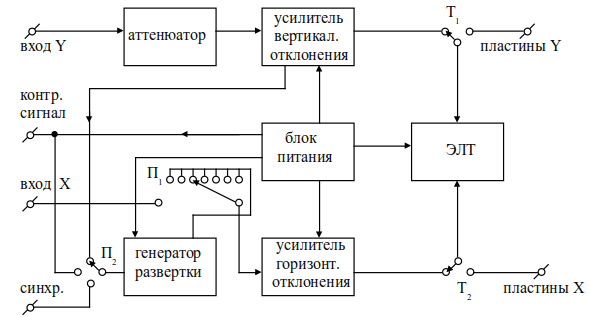
\includegraphics[width=\textwidth]{chem.png}
	\caption{Упрощенная блок-схема осциллографа}
	\label{fig:chem}
\end{figure}

Основным элементом электронного осциллографа является электронно-лучевая трубка.

\subsection{ЭЛТ осциллографа}

Электронно-лучевая трубка (рис. \ref{fig:elt}) представляет собой стеклянный баллон с тщательно откаченным воздухом с металлическими электродами.

\begin{figure}[H]
	\centering
	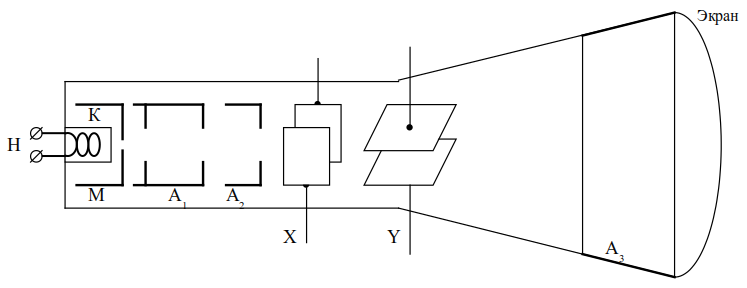
\includegraphics[width=\textwidth]{elt.png}
	\caption{Чертеж электронно-лучевой трубки осциллографа С1-1}
	\label{fig:elt}
\end{figure}

Основными частями трубки являются:
\begin{enumerate}
	\item электронная пушка
		\begin{enumerate}
			\item подогревный катод
			\item модулятор
			\item 1-й анод
			\item 2-й анод
		\end{enumerate}
	\item флуоресцирующий экран
	\item отклоняющие пластины
\end{enumerate}

Электронная пушка создает поток электронов и формирует этот поток в электронный луч.

Электронный луч, состоящий из быстро летящих электронов, направляется на флуоресцирующий экран.

Первый и второй аноды $A_1$ и $A_2$ имеют положительный потенциал относительно катода. Потенциал $A_2$ делается выше (1 -- 2 кВ), чем потенциал $A_1$ (от 100 -- 200 В). 

Конфигурация и взаимное расположение анодов подбирается таким образом, что электрическое поле, действующее на электроны, ускоряет их и собирает в тонкий луч. 

Действие электрического поля на поток электронов аналогично фокусированию светового потока оптической линзой.

Чем больше электронов в пучке, тем ярче будет пятно на экране. Величина тока в пучке регулируется напряжением на модуляторе. Фокусировка осуществляется изменением напряжения на первом аноде (изменяется конфигурация электрического поля и его фокусирующее действие).

Отклонение электронного луча производится с помощью электрических полей, создаваемых между парами взаимно-перпендикулярных отклоняющих пластин. 

Для получения на экране формы исследуемого напряжения -- осциллограммы, необходимо исследуемое напряжение подавать на вертикальные пластины, а по горизонтали заставить луч смещаться равномерно по времени, для чего на горизонтальные пластины подается пилообразное напряжение, снимаемое с генератора развертки.

Важным параметром трубки является ее чувствительность 

\begin{equation}
	\label{f:kappa}
	\varkappa=\frac{l_1l_2}{U_{A2}d}
\end{equation}

\subsection{Блок развертки}

Пилообразное напряжение, с помощью которого осуществляется равномерное во времени отклонение луча в горизонтальном направлении, вырабатывается генератором развертки.

Реальный ход изменения напряжения развертки, т.е. напряжения на конденсаторе, происходит, согласно теории электрических цепей, по экспоненциальному закону. Поэтому для получения подобного пилообразному напряжения можно брать только небольшой участок экспоненты, где она несильно отличается от прямой (рис. \ref{fig:exp}).

\begin{figure}[H]
	\centering
	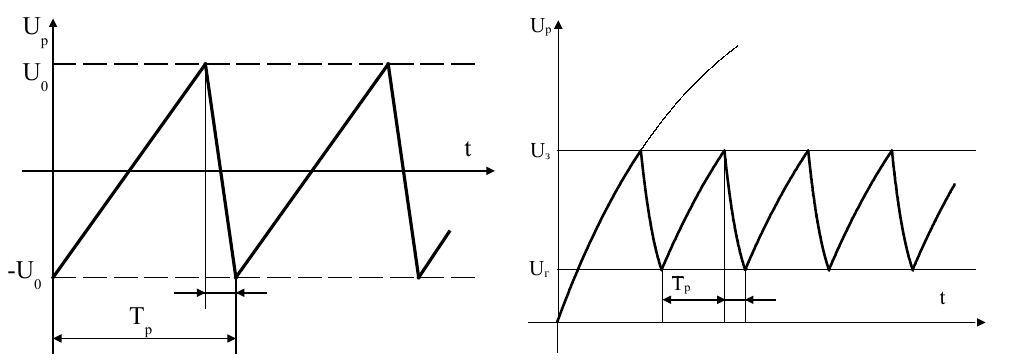
\includegraphics[width=1\textwidth]{exp.png}
	\caption{Теоретическое пилообразное напряжение и реальное скалообразное}
	\label{fig:exp}
\end{figure}

Генератор собран на газонаполненной лампе -- тиратроне, которая имеет накаливаемый катод и управляющую сетку. 

Пока напряжение на аноде тиратрона не достигнет определенной величины, носящей название напряжения зажигания $U_\text{з}$, тиратрон практически не пропускает ток. 

В это время конденсатор, включенный между анодом и катодом тиратрона, заряжается от источника через резистор. 

Как только напряжение на конденсаторе (а, следовательно, и на аноде тиратрона) достигнет величины $U_\text{з}$, тиратрон «зажигается», его сопротивление резко падает, и конденсатор быстро разряжается через тиратрон. 

Разряд длится до тех пор, пока напряжение на конденсаторе (и на аноде тиратрона) не упадет до величины напряжения «гашения» $U_\text{г}$. 

Тиратрон при этом закрывается, его сопротивление резко возрастает, а конденсатор вновь начинает заряжаться до величины $U_\text{з}$ и т.д. 

Графическая иллюстрация этого процесса приведена на (рис. \ref{fig:exp}). 

Легко понять, что осциллограмма будет устойчивой, если период напряжения развертки кратен периоду напряжения исследуемого сигнала, т.е. при условии:
\begin{equation}
	\Tr=n\cdot\Ts,
\end{equation}
где $n$ -- целое число.

Для получения неподвижной осциллограммы достаточно выполнения менее жесткого условия 
\begin{equation}
	m\cdot\Tr=n\cdot\Ts,
\end{equation}
где $m$ и $n$ -- целые числа. 

Правда, в этом случае может получиться наложение друг на друга разных кусков осциллограммы. Например, для случая m = 2, n = 3 сигнал будет выглядеть так (для наглядности показан обратный ход луча):
\begin{figure}[H]
	\centering
	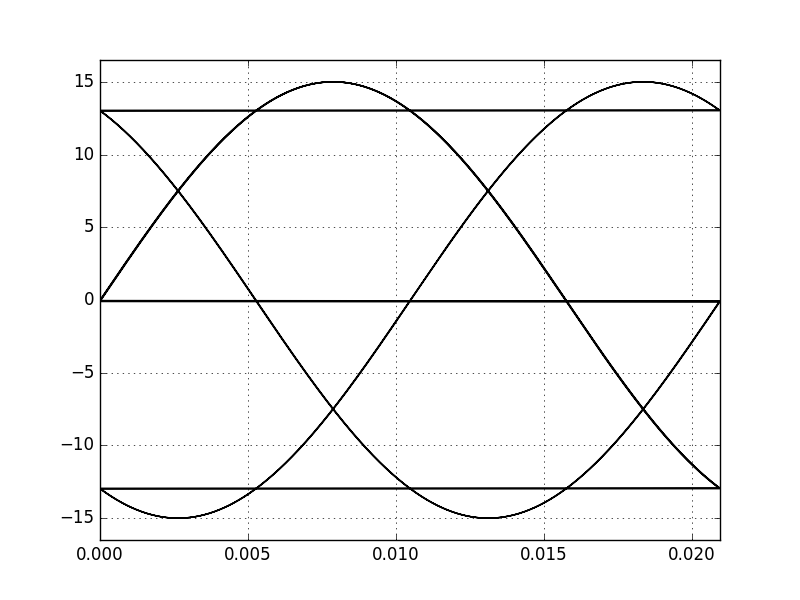
\includegraphics[width=0.8\textwidth]{freq-3-2-cross.png}
	\caption{Сигнал на экране осциллографа при $2\Tr=3\Ts$}
	\label{fig:cross}
\end{figure}

Глаз не будет видеть движение луча, если время послесвечения трубки -- время свечения экрана после прекращения возбуждения его электронным лучом -- больше перида развертки, и на экране будет видна сплошная линия. 

Заметим также, что во время обратного хода на модулятор трубки поступает отрицательное напряжение, запирающее луч, поэтому обратный ход луча на экране трубки не виден.

%%%%%%%%%%%%%%%%%%%%%%%%%%%%%%%%%%%%%%%%%%%%%%%%%%%%%%%%%%%%%
%%%%%%%%%%%%%%%%%%%%%%%%%%%%%%%%%%%%%%%%%%%%%%%%%%%%%%%%%%%%%

\newpage
\section{Изучение осциллографа}

\subsection{Определение величины чувствительности вертикального и горизонтального каналов осциллографа}

При измерениях частота генератора выставлена на $1000$ Гц, ослабление сигнала -- <<$1:1$>>.

Расчет ведется по формуле 
\begin{equation}
	\varkappa=\frac{h}{2\sqrt{2}U}
\end{equation}

Класс точности вольтметра $2.5$, для максимального значения шкалы $1.5$ вольт $\Delta{U_1}=2.5\cdot1.5/100=0.0375$ В, для максимального значения шкалы $15\cdot10^{-3}$ вольт $\Delta{U_2}=2.5\cdot15\cdot10^{-3}/100=0.000375$ В.

Приборная погрешность при измерении длины --- $\Delta{h}=1$ мм.

\begin{gather}
	\varepsilon(\varkappa)=\frac{\Delta{h}}{h}+\frac{\Delta{U}}{U}\\
	\Delta(\varkappa)=\frac{h}{2\sqrt{2}U}\cdot(\frac{\Delta{h}}{h}+\frac{\Delta{U}}{U})
\end{gather}

\begin{table}[H]
	\centering
	\begin{tabu} to \textwidth {|X[1c]|X[1.5c]|*{3}{X[c]|}X[1.5c]|} 
		\hline
		\multirow{4}{*}{\vspace{1em}Y-канал} & $U$, В & $9\cdot10^{-3}$ & $12\cdot10^{-3}$ & $13\cdot10^{-3}$ & \multirow{3}{*}{\vspace{1.5em} $U_{max}$ шкалы, В } \\ 
		\hhline{|~|-|-|-|-|~|}
		 & $h$, мм & 26 & 34 & 36 & \\
		 \hhline{|~|-|-|-|-|~|}
		 & $\varkappa$, мм/в & $1021.38\pm81$ & $1001.734\pm60$ & $979.07\pm50$ & \\[1ex]
		 \hhline{|~|-|-|-|-|-|}
		 & $\varkappa_\text{ср}$, мм/в & \multicolumn{3}{c|}{$1000.72\pm65$} & $15\cdot10^{-3}$\\ 
		 \hline
	\end{tabu}
	\label{tab:kappa-vert}
	\caption{Вертикальный канал усиления}
\end{table}
\begin{table}[H]
	\centering
	\begin{tabu} to \textwidth {|X[1c]|X[1.5c]|*{3}{X[c]|}X[1.5c]|} 
		\hline
		\multirow{4}{*}{\vspace{1em}X-канал} & $U$, В & $0.9$ & $1.2$ & $1.3$ & \multirow{3}{*}{\vspace{1.5em} $U_{max}$ шкалы, В } \\ 
		\hhline{|~|-|-|-|-|~|}
		 & $h$, мм & 34 & 48 & 52 & \\
		 \hhline{|~|-|-|-|-|~|}
		 & $\varkappa$, мм/в & $13.35\pm0.94$ & $14.14\pm0.73$ & $14.14\pm0.67$ & \\[1ex]
		 \hhline{|~|-|-|-|-|-|}
		 & $\varkappa_\text{ср}$, мм/в & \multicolumn{3}{c|}{$13.87\pm0.79$} & $1.5$\\ 
		 \hline
	\end{tabu}
	\label{tab:kappa-hor}
	\caption{Горизонтальный канал усиления}
\end{table}

\subsection{Срыв синхронизации при изменении частоты генератора}

\begin{table}[H]
	\centering
	\begin{tabu} to \textwidth {|X[1c]|X[2c]|*{2}{X[c]|}X[1.5c]|} 
		\hline
		$\frac{n}{m}$ & Амплитуда синхронизации, дел& $-\Delta{f}$, Гц & $+\Delta{f}$, Гц & $\Delta{f_\text{ср}}$, Гц \\ 
		\hline
		\multirow{2}{*}{$1$}& $2$ & 3 & 3 & 3\\
		\hhline{|~|-|-|-|-|}
		& $9$ & 10.5 & 20 & 15.25\\
		\hline
		%
		\multirow{2}{*}{$\frac{1}{2}$}& $2$ & 2 & 1.5 & 1.75\\
		\hhline{|~|-|-|-|-|}
		& $9$ & 4 & 2 & 3\\
		\hline
		%
		\multirow{2}{*}{$2$}& $2$ & 1 & 1.5 & 1.25\\
		\hhline{|~|-|-|-|-|}
		& $9$ & 20 & 45 & 32.5\\
		\hline
	\end{tabu}
	\label{tab:kappa-hor}
	\caption{Срыв синхронизации при изменении частоты генератора}
\end{table}

Из опыта следует, что синхронизация лучше (больше синхронизируемое отклонение от частоты, кратной частоте сигнала) для $\frac{n}{m}=2$, нежели чем для $\frac{n}{m}=1$, т.е. два периода на экране синхронизируются лучше, чем один.

\subsection{Время послесвечения трубки}

Оценка времени послесвечения трубки определялась частотой, при которой получаемая глазом картина с экрана  переставала оцениваться как отдельные кадры. Подбор частоты дал такое значение $f_\text{с}=43$ Гц, откуда время послесвечения $T=\frac{1}{f_\text{с}}$ секунды, $\approx0.0232$ секунды.


\newpage
\subsection{Линейность вертикального канала усиления}

Вертикальный канал усиления должен обладать хорошей линейностью, чтобы не искажать формы исследуемого напряжения. 

Так как отклонение на экране пропорционально напряжению, то можно замерить линейность канала усиления, подавая известное напряжение на вход усилителя и замеряя отклонение луча (отражает амплитуду сигнала на выходе из усилителя).

\begin{figure}[H]
	\centering
	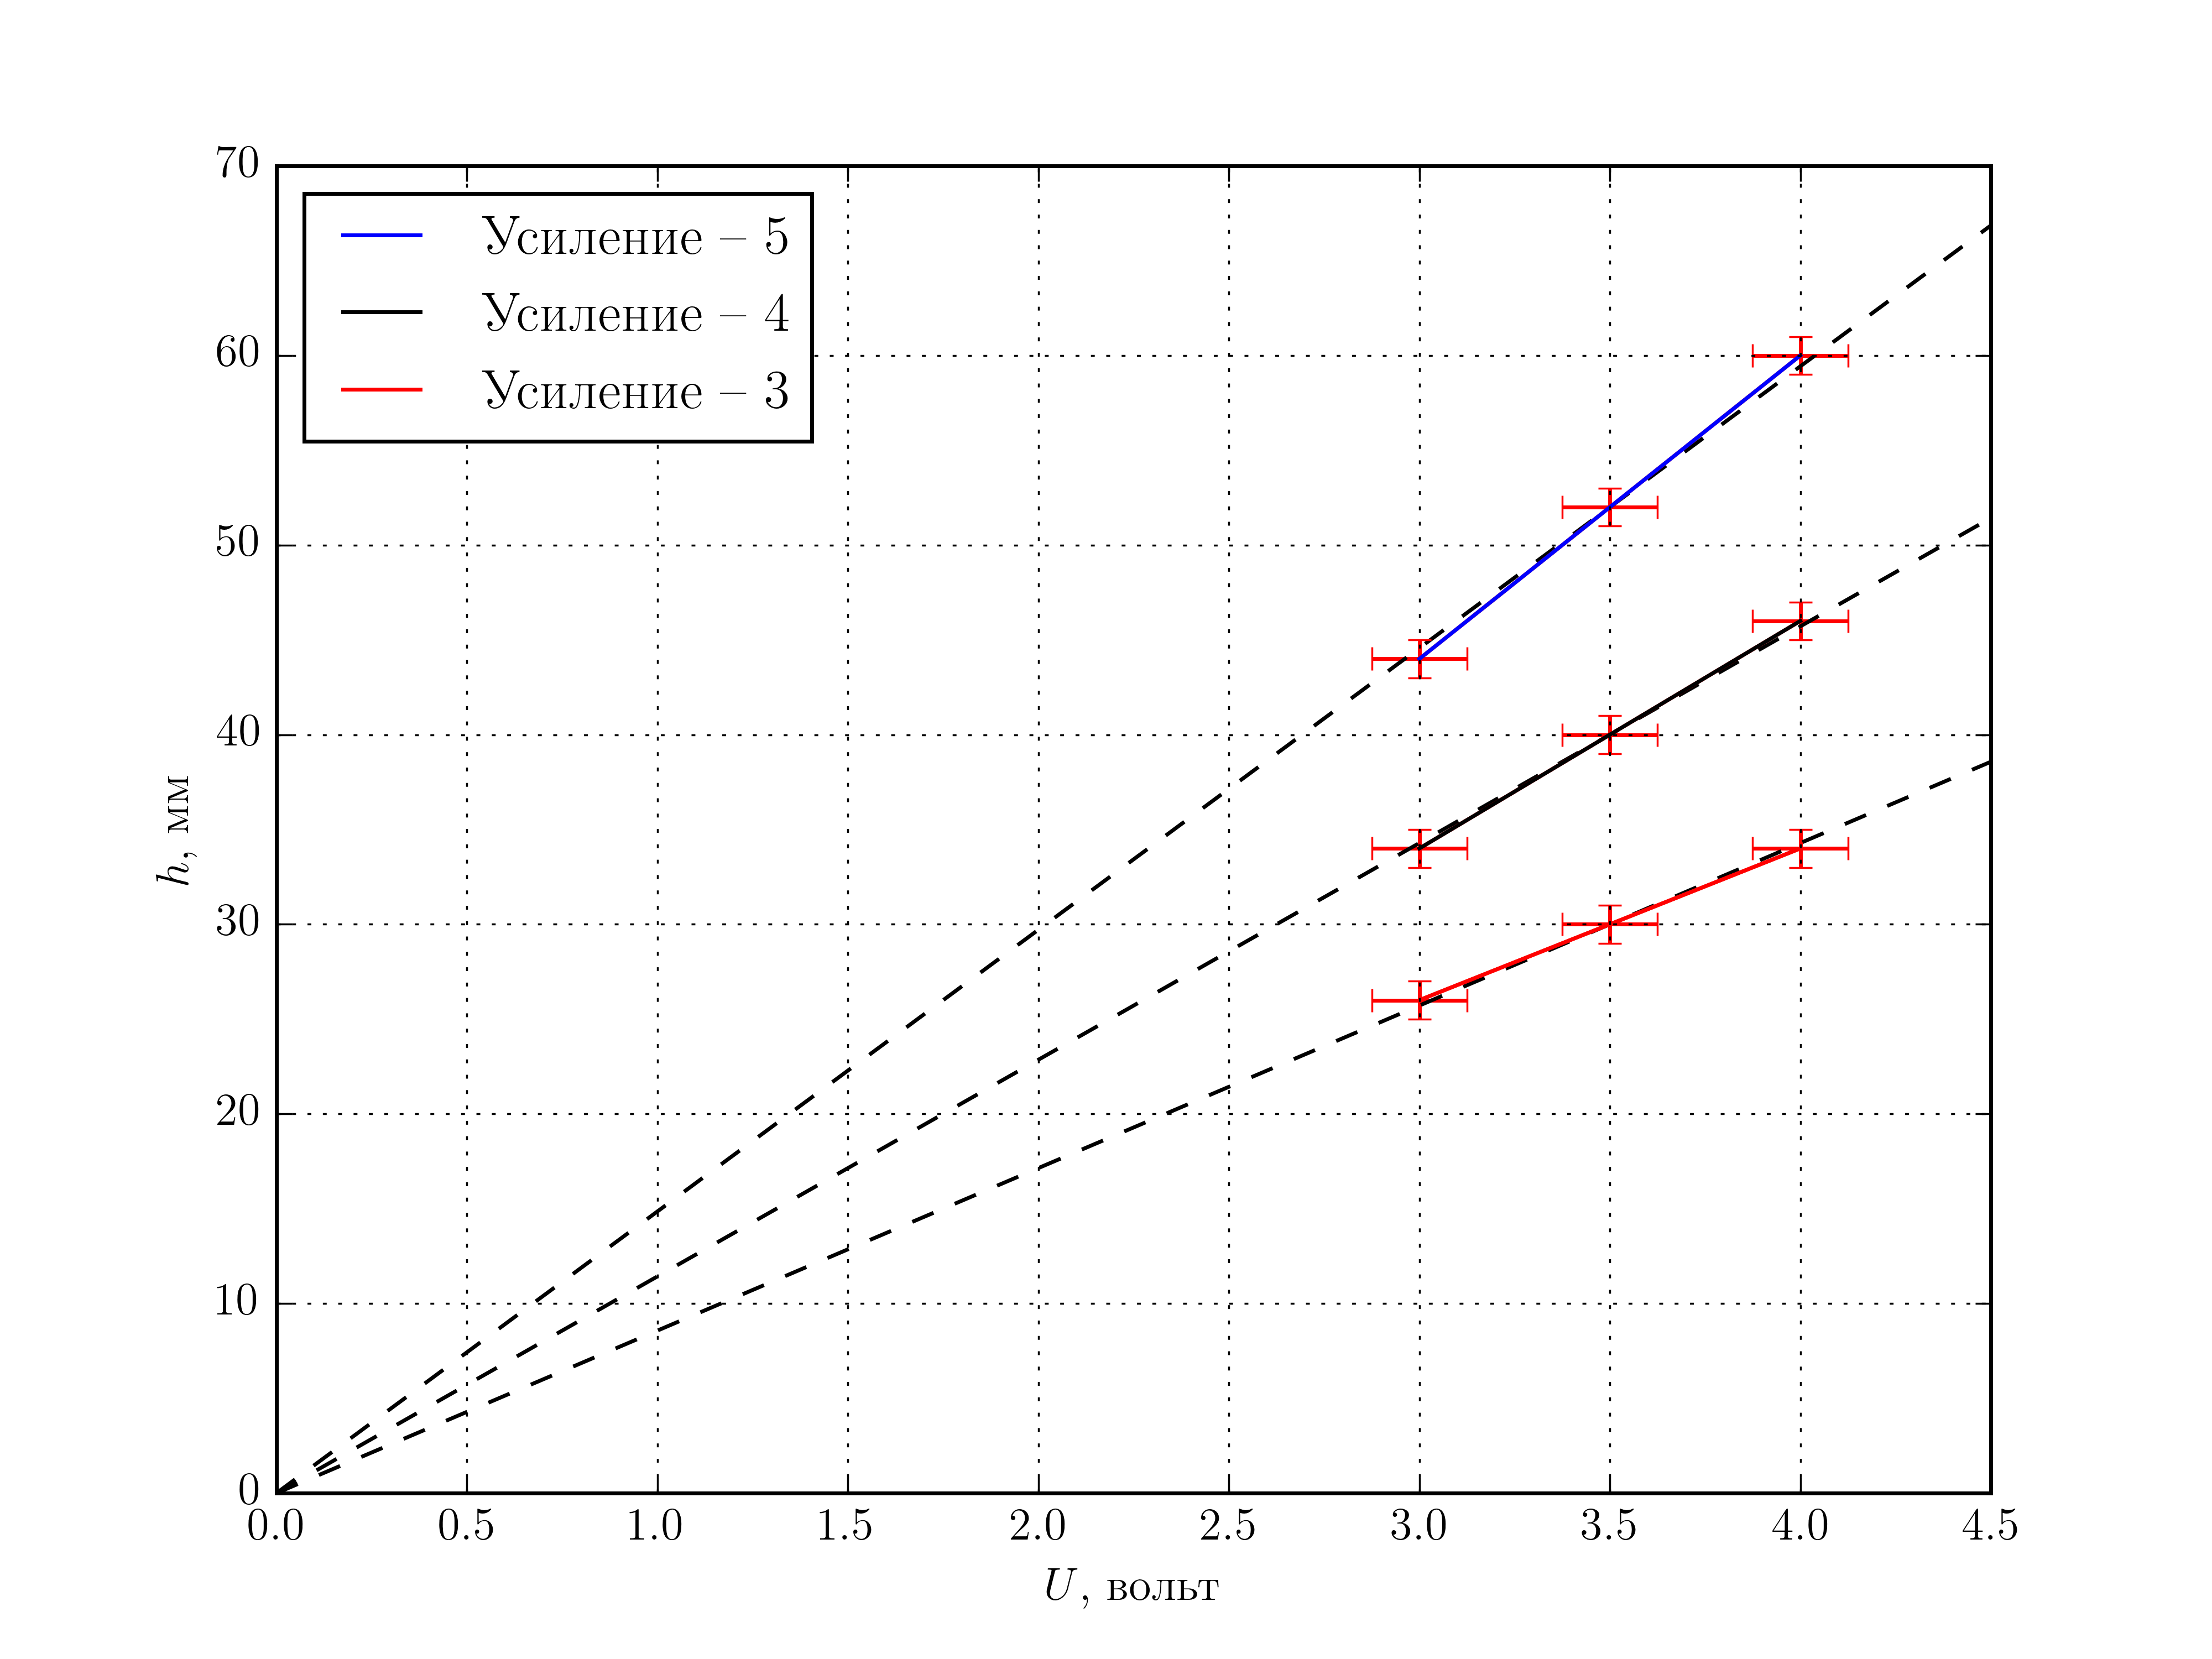
\includegraphics[width=1\textwidth]{linear.png}
	\caption{Линейность вертикального канала усиления. Значения усиления: $3,4,5$}
	\label{fig:linear}
\end{figure}

Видно, что на усилении 5 наблюдается искажение, однако, лежащее в пределах погрешности - это может быть линейным искажением сигнала усилителя.

\label{ss:freq}\subsection{Частотные свойства вертикального канала усиления}

Вертикальный канал усиления, кроме линейности, должен также иметь хорошие частотные характеристики, чтобы не искажать сигнал и иметь возможность исследовать сигналы высоких частот. 

Замер частотных свойств производился подачей сигнала разной частоты - от $100$ Гц до $200$ кГц. На частоте порядка $1$ кГц происходит спад АЧХ. Главной причиной спада являются ограниченные частотные свойства активных элементов усилителя.

На графике (рис. \ref{fig:freq-stats}) приведена также теоретическая зависимость отклонения луча от частоты сигнала, отражающая АЧХ электронно-лучевой трубки.

\begin{figure}[H]
	\centering
	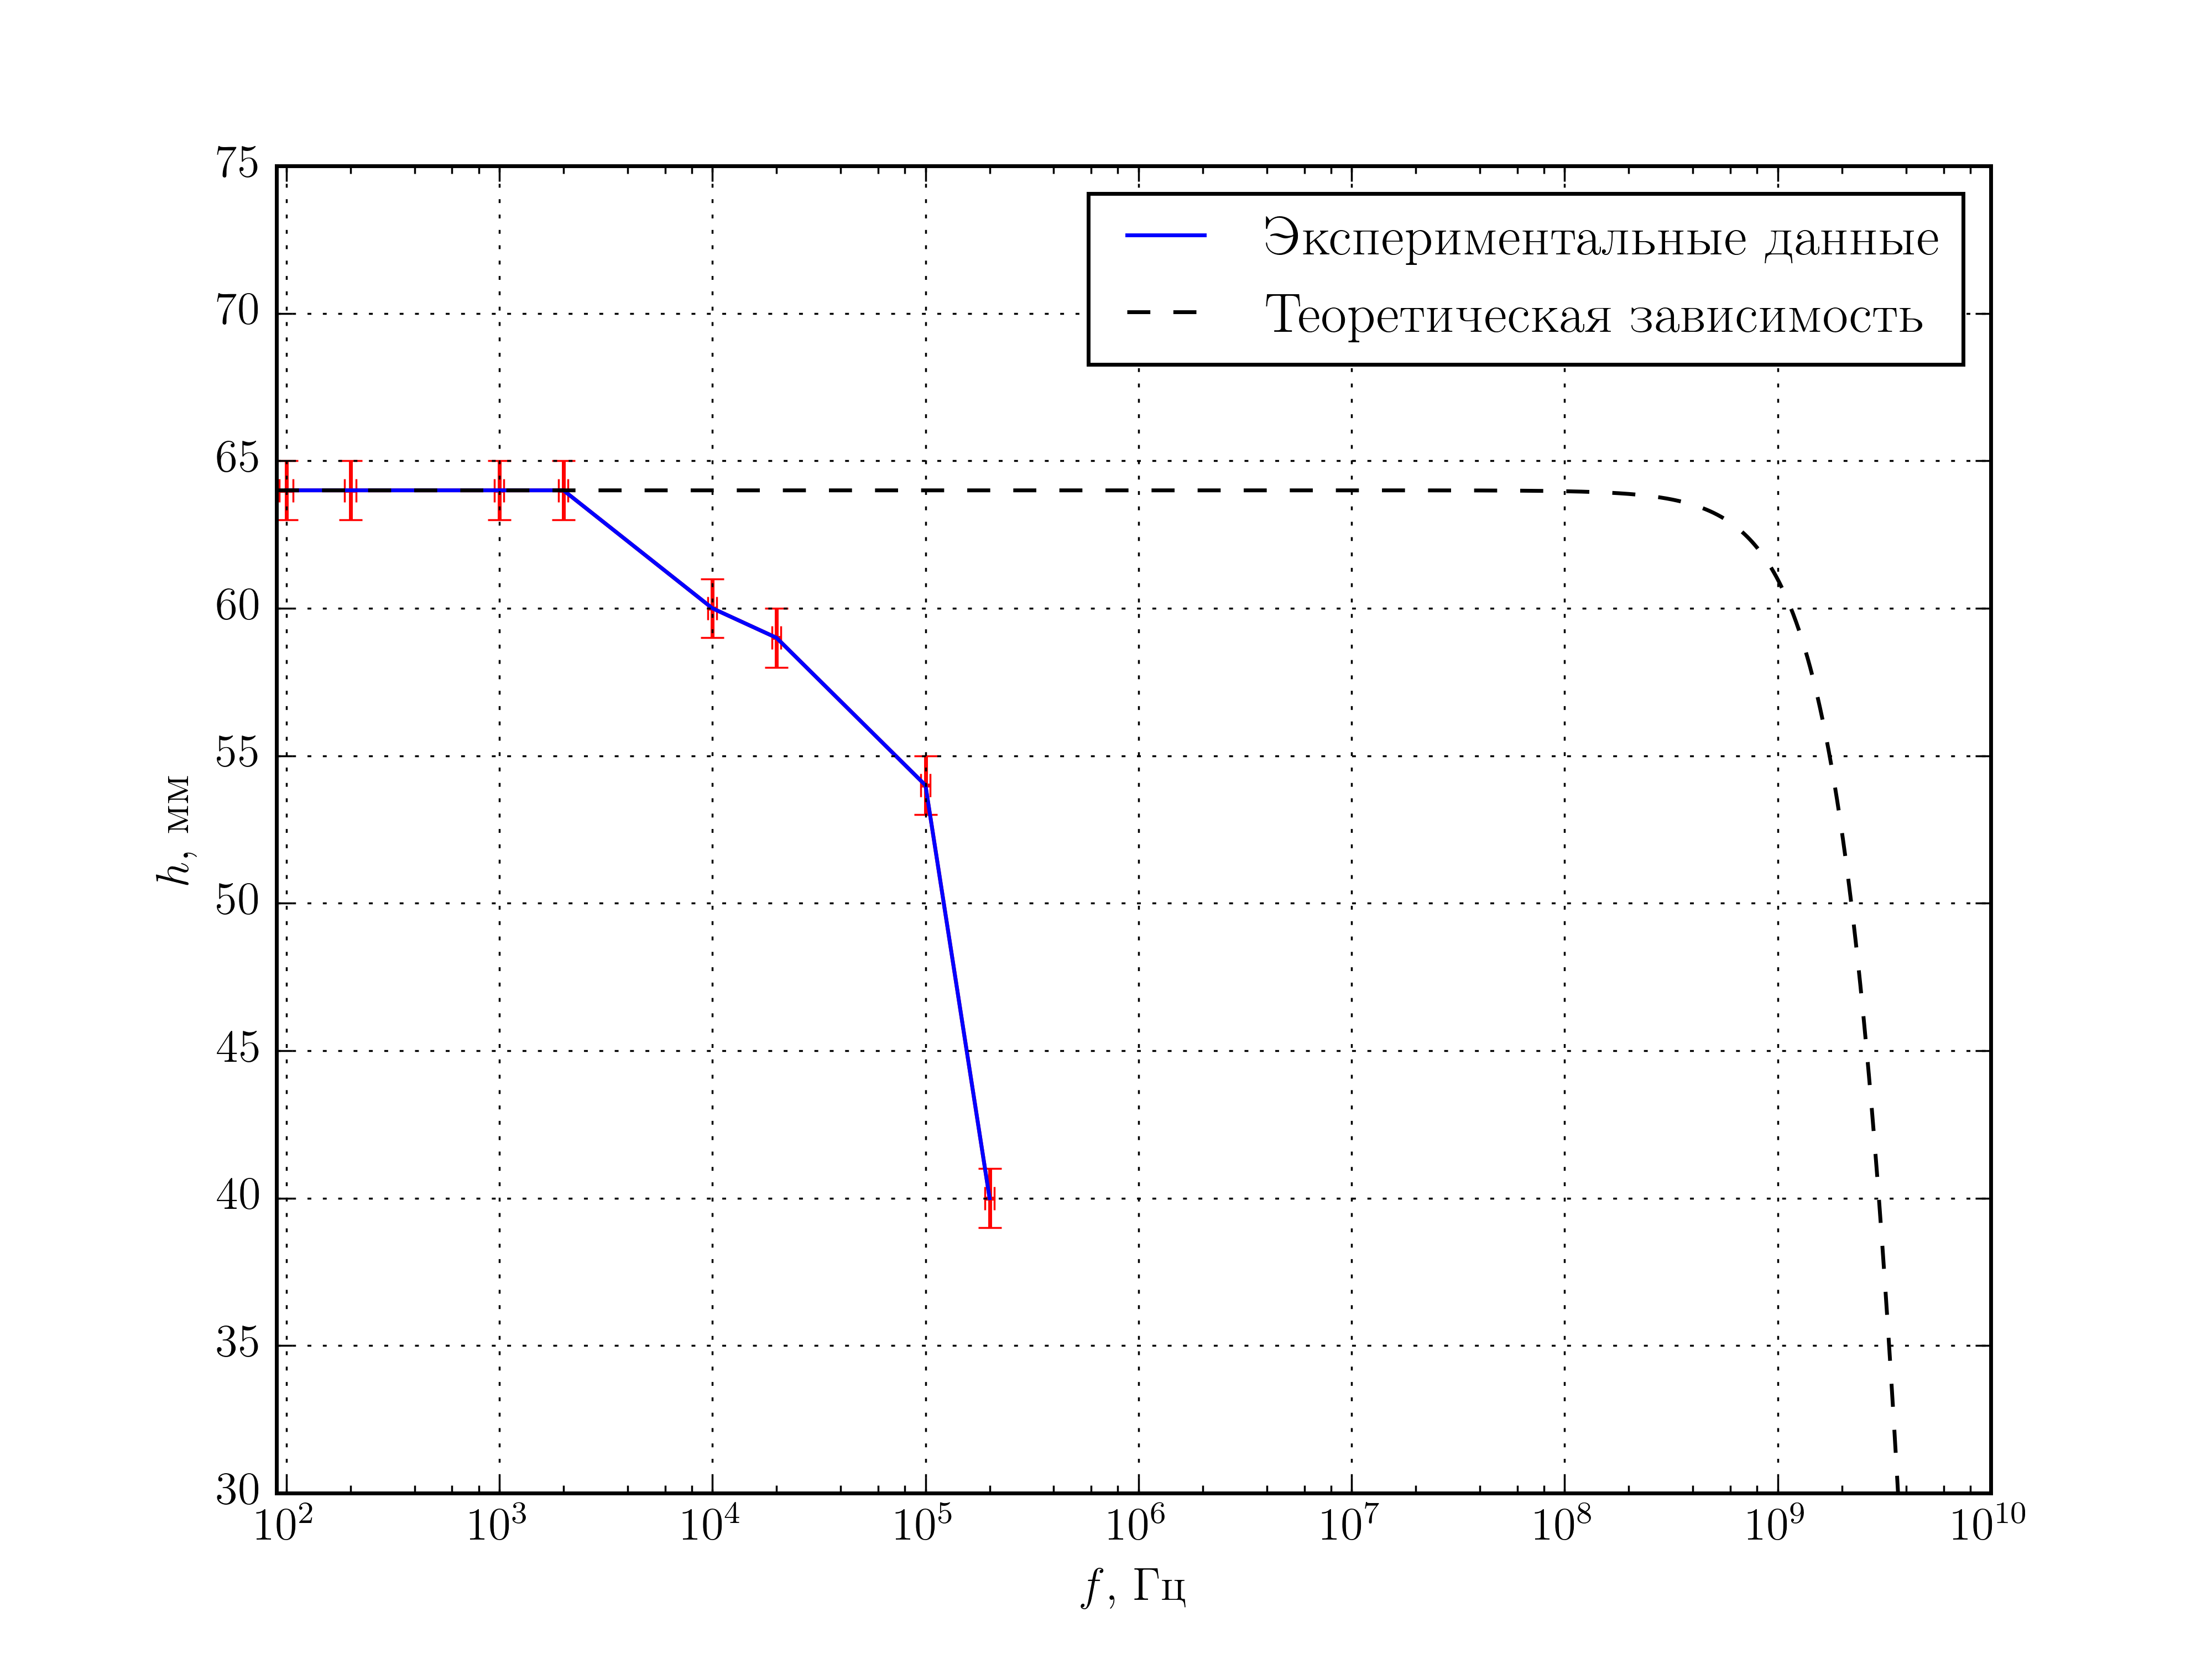
\includegraphics[width=1\textwidth]{freq-stats.png}
	\caption{АЧХ вертикального канала усиления}
	\label{fig:freq-stats}
\end{figure}

\subsubsection{Вывод АЧХ трубки}

\begin{gather}
	a=\frac{e}{m}U_0\cos(\omega{t}+\phi_0)\\
	\eta=\frac{e}{m}\\
	v_y=\int_0^t adt=\frac{\eta{U_0}}{d\omega}\sin(\omega{t}+\phi_0)\bigg|_0^t=\frac{\eta{U_0}}{d\omega}\left[\sin(\omega{t}+\phi_0)-\sin\phi_0\right]=\\
	\label{eq:cos}=\frac{2\eta{U_0}}{d\omega}\sin(\frac{\omega{t}}{2})\cdot\cos(\omega{t}/2+\phi_0)
\end{gather}
Тогда можем найти скорость $v_y$ на вылете из пластин. Введем время пролета через пластины $t=l_1/v_x$, время пролета до экрана от пластин $\tau=l_2/v_x$.

При этом $v_x$ можем найти из ЗСЭ:
\begin{equation}
	\frac{mv^2_x}{2}=eU_A\Longrightarrow v_x=\sqrt{2\eta{U_A}}
\end{equation}

Тогда можем записать $h=v_y(t=\frac{l_1}{v_x})\cdot\tau$, учитывая максимальное значение косинуса в (\ref{eq:cos}) равным 1:
\begin{gather}
	h=\frac{2\eta{U_0}}{d\omega}\sin\left(\frac{\omega{l_1}}{2v_x}\right)\cdot\frac{l_2}{v_x\cdot\omega}
\end{gather}

и окончательный ответ
\begin{gather}
	h=\frac{2\eta{U_0}l_2}{d\sqrt{2\eta{U_A}}}\frac{\sin\left(\omega\frac{{l_1}}{2\sqrt{2\eta{U_A}}}\right)}{\omega}
\end{gather}


\newpage
\section{Работа развертки осциллографа}

При минимальном значении напряжения луч находится в крайнем левом положении на горизонтальной прямой экрана. По мере роста пилообразного напряжения луч перемещается слева направо с почти постоянной скоростью.

Луч за время прямого хода tпр переместится в крайнее правое положение экрана.  Когда напряжение спадает, луч совершает обратный ход — луч быстро возвращается в исходное положение, чтобы в следующий период повторить цикл, состоящий из прямого и обратного хода.

Чтобы линия развертки или изображение сигнала не мерцали при наблюдении, луч должен прочерчивать одну и ту же траекторию не менее 25-30 раз в секунду. 

При этом используется инерционная способность человеческого глаза сохранять зрительное впечатление примерно 1/15 с. Расчитанное для данного осциллографа время послесвечения ---- 1/43 с, т.е. для немерцающей траектории необходимо, чтобы луч вернулся в ранее пройденную точку не позже, чем через 1/43 секунды (частота 43 Гц).

\subsection{Осциллограмма сигнала}
\begin{figure}[H]
	\centering
	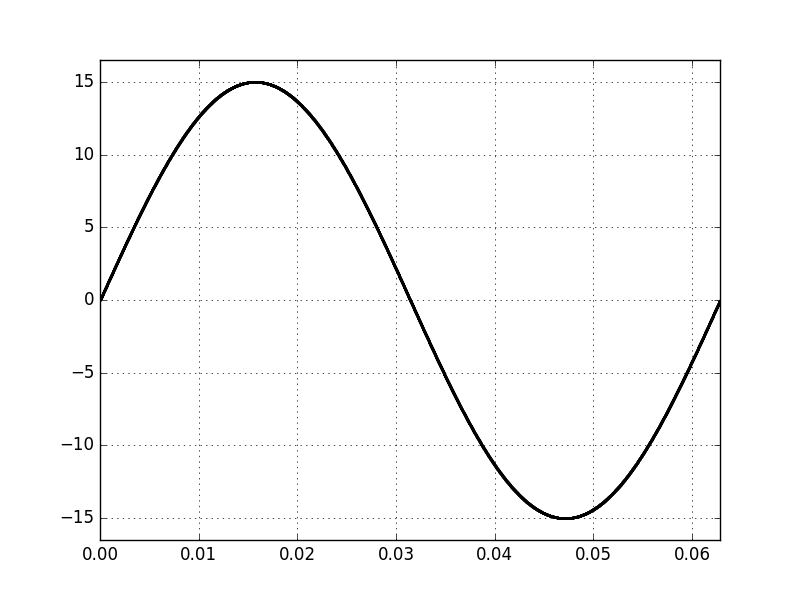
\includegraphics[width=0.85\textwidth]{freq-1-1.png}
	\caption{Осциллограмма сигнала для $\frac{m}{n}=\frac{1}{1}$}
	\label{fig:freq-1-1}
\end{figure}

\begin{figure}[H]
	\centering
	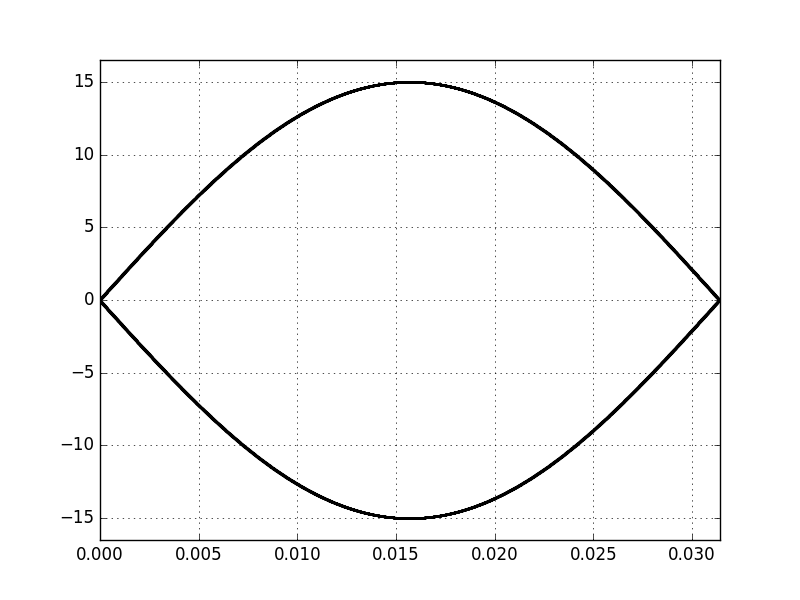
\includegraphics[width=0.85\textwidth]{freq-1-2.png}
	\caption{Осциллограмма сигнала для $\frac{m}{n}=\frac{1}{2}$}
	\label{fig:freq-1-2}
\end{figure}

\begin{figure}[H]
	\centering
	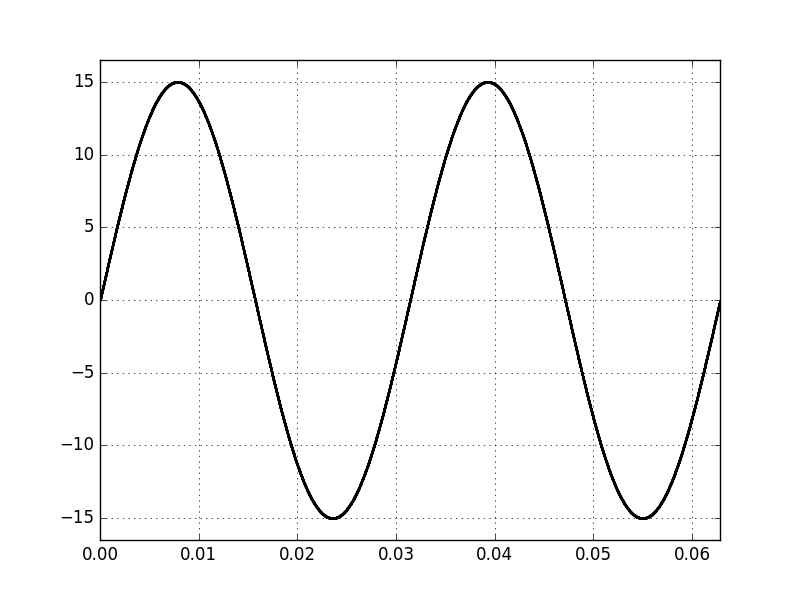
\includegraphics[width=0.85\textwidth]{freq-2-1.png}
	\caption{Осциллограмма сигнала для $\frac{m}{n}=\frac{2}{1}$}
	\label{fig:freq-2-1}
\end{figure}

\begin{figure}[H]
	\centering
	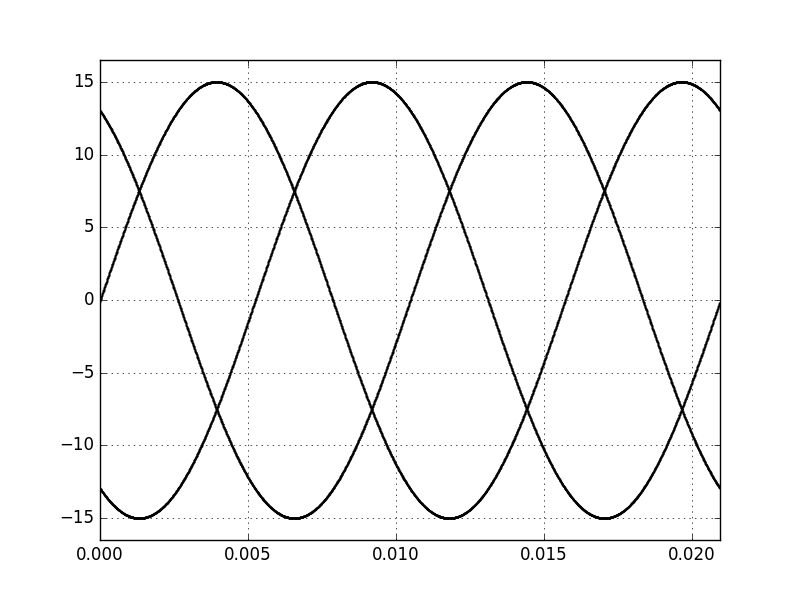
\includegraphics[width=0.85\textwidth]{freq-3-4.png}
	\caption{Осциллограмма сигнала для $\frac{m}{n}=\frac{3}{4}$}
	\label{fig:freq-3-4}
\end{figure}

\begin{figure}[H]
	\centering
	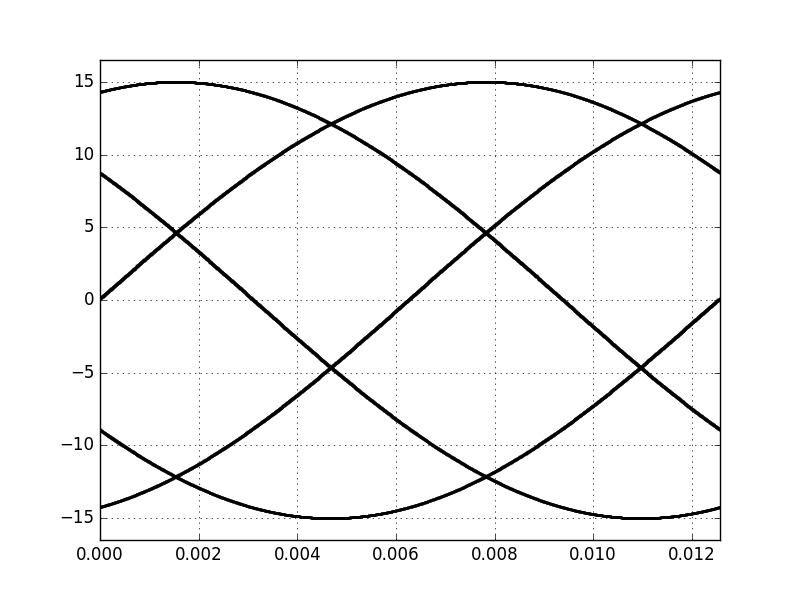
\includegraphics[width=0.85\textwidth]{freq-5-2.png}
	\caption{Осциллограмма сигнала для $\frac{m}{n}=\frac{5}{2}$}
	\label{fig:freq-5-2}
\end{figure}


\subsection{Бег осциллограммы}
\def\Tr{T_\text{р}}
\def\Ts{T_\text{с}}
При небольшой расстройке частот на осциллографе можно наблюдать движение (бег) несинхронизированной осциллограммы влево или вправо. 

Это явление легко иллюстрируется построением траектории движения луча по экрану в цикле развёртки. 

Если период развертки не равен периоду исследуемого сигнала, то график строится со сдвигом, причем если $\Tr<\Ts$, то сдвиг положительный (рис. \ref{fig:freq-1-0.95}).

В противном случае, если $\Tr>\Ts$, сдвиг то отрицательный  (рис. \ref{fig:freq-1-1.05}).

Отрисовка периодического сигнала со сдвигом создает иллюзию <<бега>> осциллограммы соответственно влево для отрицательного сдвига и вправо для положительного.

\begin{figure}[H]
	\centering
	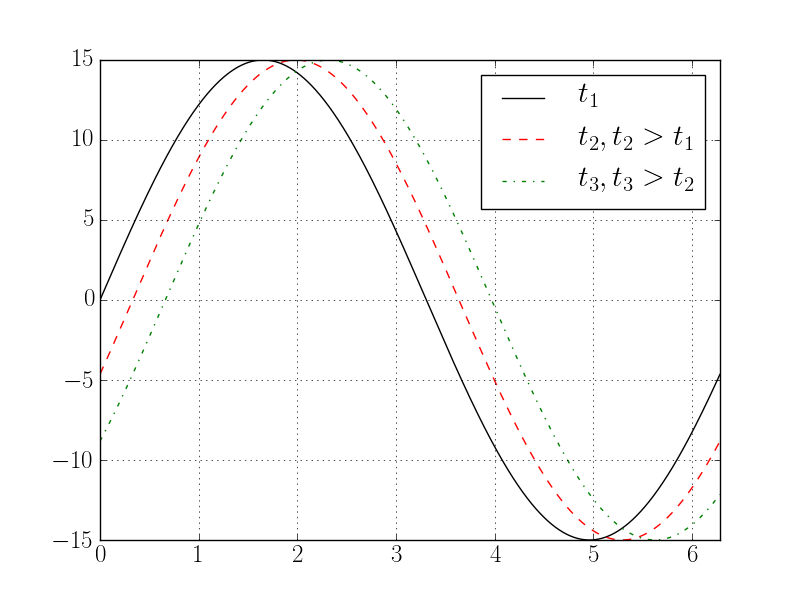
\includegraphics[width=0.85\textwidth]{freq-1-095.png}
	\caption{Бегущая развертка при $\frac{m}{n}=\frac{1}{0.95}$}
	\label{fig:freq-1-0.95}
\end{figure}
\begin{figure}[H]
	\centering
	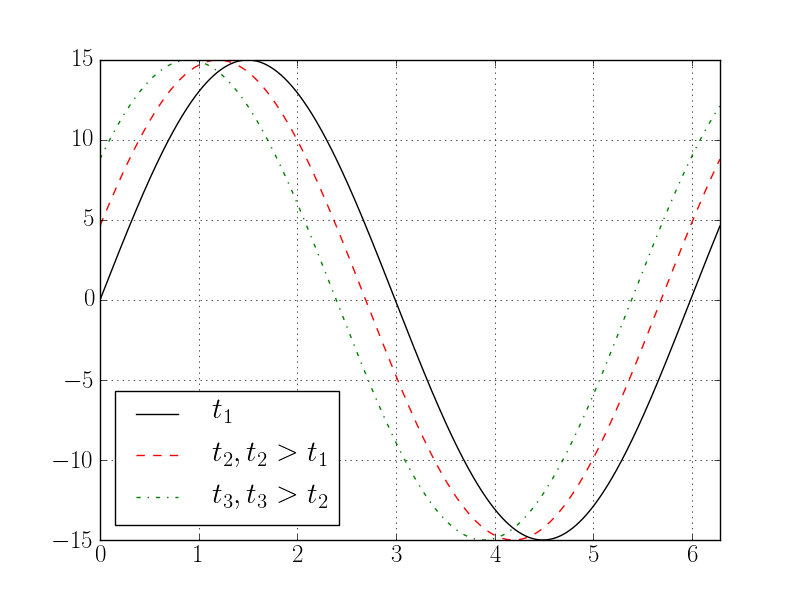
\includegraphics[width=0.85\textwidth]{freq-1-105.png}
	\caption{Бегущая развертка при $\frac{m}{n}=\frac{1}{1.05}$}
	\label{fig:freq-1-1.05}
\end{figure}
\subsection{Фигуры Лиссажу}
\begin{figure}[H]
	\centering
	% \hspace{-1cm}	
	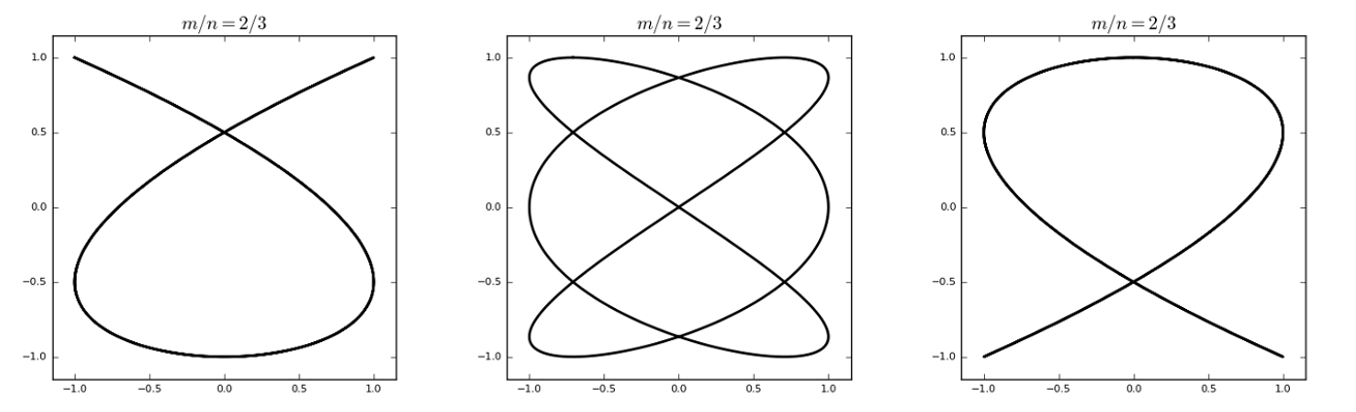
\includegraphics[width=0.85\textwidth]{lissajous2-3.png}
	\caption{Фигуры Лиссажу для $\frac{m}{n}=\frac{3}{2}$}
	\label{fig:lissajous-2}
\end{figure}
\begin{figure}[H]
	\centering
	% \hspace{-1cm}	
	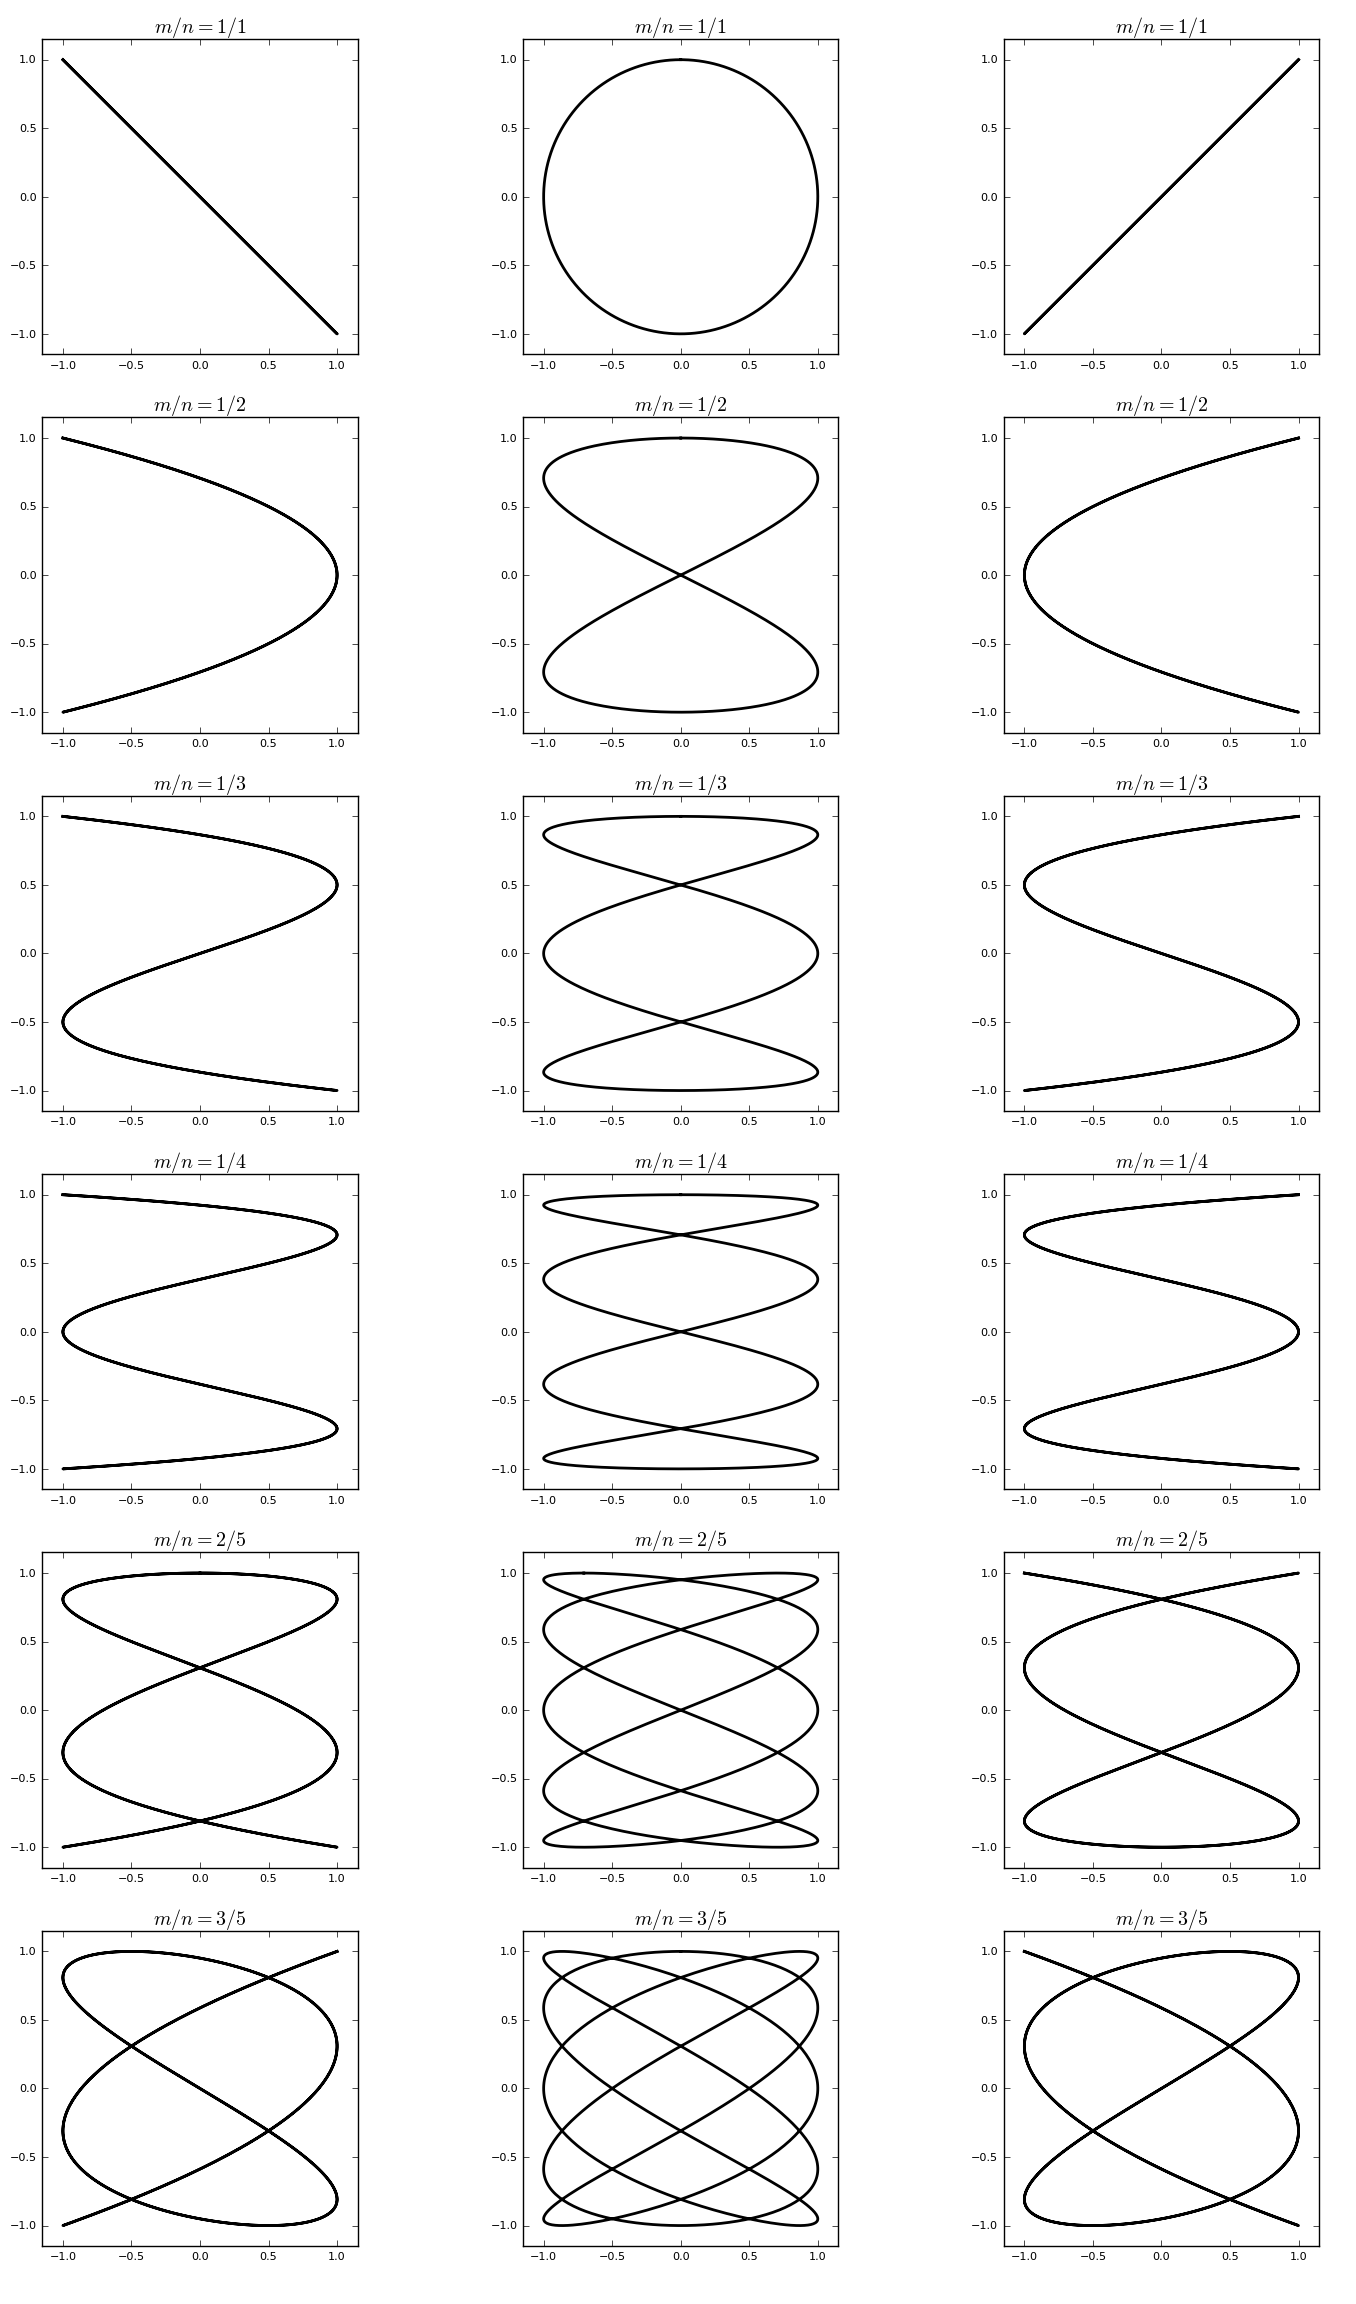
\includegraphics[width=0.8\textwidth]{lissajous3.png}
	\caption{Фигуры Лиссажу для $\frac{m}{n}=1;2;3;4;\frac{5}{2};\frac{5}{3}$}
	\label{fig:lissajous-1}
\end{figure}
\section{Зоны синхронизации}
\begin{figure}[H]
	\centering
	% \includegraphics[]{}	
	\begin{tikzpicture}
	\hspace{-1cm}
		\draw[fill,yellow!60] 	
	% (1.5,0) --
	(0,0) --
	(3.0000,1.0000) --
	(4.5000,2.0000) --
	(6.0000,3.0000) --
	(6.7500,4.0000) --
	(7.5000,5.0000) --
	(9.0000,6.0000) --
	(9.7500,7.0000) --
	(10.5000,8.0000) --
	(12,\lft) --
	(\rft,\lft) --
	(\rft,-\lft) --
	(15.0000,-8.0000) --
	(13.5000,-7.0000) --
	(10.5000,-6.0000) --
	(9.0000,-5.0000) --
	(6.7500,-4.0000) --
	(5.2500,-3.0000) --
	(3.7500,-2.0000) --
	(2.2500,-1.0000) -- cycle;
			

\draw[step=.1cm , gray!20] (0,-\lft) grid (\rft ,\lft);
\draw[step=0.5cm , gray!50] (0,-\lft) grid (\rft ,\lft);
\draw[step=1cm , gray!80] (0,-\lft) grid (\rft ,\lft);


\draw[-{>[scale=1.0]}] (-0,0) -- (10*1.5 +1 ,0) node[anchor=north west] {\scalebox{1.5}{$A$}};
\draw[->] (0,-\lft) -- (0,\lft+1 ) node[anchor=east] {\scalebox{1.5}{$\frac{\nu_\text{с}-\nu_\text{р}}{\nu_\text{р}}$}};


\foreach \x in {1,2,3,4,5,6,7,8,9,10} {
	\draw (\x*\Xstep,0.05) -- (\x*\Xstep,-0.05);
	\draw (\x*\Xstep,0) node[anchor=north] {\scalebox{1.5}{$\x$}};
}

\foreach \y in {-0.3,-0.2,-0.1, 0, 0.1,0.2,0.3} {
	\draw (0.05,\y*\Ystep) -- (-0.05,\y*\Ystep);
	\draw (0,\y*\Ystep) node[anchor=east] {\scalebox{1.5}{$\y$}};
}

% \draw[blue] (15,0.5) node[anchor=east] {\scalebox{1.4}{Синхронизованная зона}};
% \draw[blue] (9.5,8.2) node[anchor=east] {\scalebox{1.4}{Несинхронизованная зона}};
% \draw[blue] (9.5,-8.3) node[anchor=east] {\scalebox{1.4}{Несинхронизованная зона}};
\input{experience/table.out}		
	\end{tikzpicture}
	\caption{Зоны синхронизации при частоте развертки 100 Гц}
	\label{fig:regions-100}
\end{figure}
\begin{figure}[H]
	\centering
	% \includegraphics[]{}	
	\begin{tikzpicture}
	\hspace{-1cm}
		\def\Scale{1}
\def\lft{13}
\def\lftl{3.5}
\def\rft{10.43*1.5}
\def\Xstep{1.5}
\def\Ystep{1.5*20}
\def\Radius{0.1}
\def\Color{black}

\draw[fill,yellow!60] 
	(0,0)	 --
    (4.5000, 1.8000) --
    (6.0000, 3.0000) --
    (7.5000, 4.5000) --
    (9.0000, 6.0000) --
    (10.5000, 7.5000) --
    (12.0000, 9.0000) --
    (13.5000, 10.5000) --
    (15.0000, 12.0000) --
	(\rft,\lft) --
	(\rft,-\lftl) --   
	(8.5000, -\lftl) -- 
    (7.5000, -3.0000) --
    (4.5000, -1.5000) --
% 	(0,0) --
% 	(3.0000, 1.5000) --
% 	(5.2500, 3.0000) --
% 	(6.7500, 4.5000) --
% 	(8.2500, 6.0000) --
% 	(9.7500, 7.5000) --
% 	(10.5000, 9.0000) --
% 	(11.2500, 10.5000) --
% 	(12.0000, 12.0000) --
% 	%
% 	(12,\lft) --
% 	(\rft,\lft) --
% 	(\rft,0) --
% 	% (6.0000, -1.5000) --
% 	% (7.5000, -2.1000) --
						cycle;

% \draw[fill,yellow!60] 	
% % 	% (1.5,0) --
% 	(0,0) --
% 	%
% 	(6.0000, -1.5000) --
% 	(7.5000, -2.1000) --
% 	%
% 	(10,-\lftl) --
% 	(\rft,-\lftl) --
% 	(\rft,0) --
% 						cycle;
			
% \draw[] (0,0) .. controls (6,4) and (7,2) ..  (12,12);
\draw[step=.1cm , gray!20] (0,-\lftl) grid (\rft ,\lft);
\draw[step=0.5cm , gray!50] (0,-\lftl) grid (\rft ,\lft);
\draw[step=1cm , gray!80] (0,-\lftl) grid (\rft ,\lft);


\draw[-{>[scale=1.0]}] (-0,0) -- (10*1.5 +1 ,0) node[anchor=north west] {\scalebox{1.5}{$A$}};
\draw[->] (0,-\lftl) -- (0,\lft+1 ) node[anchor=east] {\scalebox{1.5}{$\frac{\nu_\text{с}-\nu_\text{р}}{\nu_\text{р}}$}};


\foreach \x in {1,2,3,4,5,6,7,8,9,10} {
	\draw (\x*\Xstep,0.05) -- (\x*\Xstep,-0.05);
	\draw (\x*\Xstep,0) node[anchor=north] {\scalebox{1.5}{$\x$}};
}

\foreach \y in {-0.1, 0, 0.1,0.2,0.3,0.4} {
	\draw (0.05,\y*\Ystep) -- (-0.05,\y*\Ystep);
	\draw (0,\y*\Ystep) node[anchor=east] {\scalebox{1.5}{$\y$}};
}

% \draw[blue] (15,0.5) node[anchor=east] {\scalebox{1.4}{Синхронизованная зона}};
% \draw[blue] (9.5,8.2) node[anchor=east] {\scalebox{1.4}{Несинхронизованная зона}};
% \draw[blue] (9.5,-8.3) node[anchor=east] {\scalebox{1.4}{Несинхронизованная зона}};
\input{experience/table_1k.out}		
	\end{tikzpicture}
	\caption{Зоны синхронизации при частоте развертки 1 кГц}
	\label{fig:regions-1000}
\end{figure}
\begin{figure}[H]
	\centering
	% \includegraphics[]{}	
	\begin{tikzpicture}
	\hspace{-1cm}
		\def\Scale{1}
\def\lft{13}
\def\lftl{3}
\def\rft{10.43*1.5}
\def\Xstep{1.5}
\def\Ystep{1.5*20}
\def\Radius{0.1}
\def\Color{black}

\draw[fill,yellow!60] 	
% 	% (1.5,0) --
	(0,0) --
% 	(12,\lft) --
% 	(\rft,-\lft) --
	(3.0000, 1.5000) --
	(5.2500, 3.0000) --
	(6.7500, 4.5000) --
	(8.2500, 6.0000) --
	(9.7500, 7.5000) --
	(10.5000, 9.0000) --
	(11.2500, 10.5000) --
	(12.0000, 12.0000) --
	%
	(12,\lft) --
	(\rft,\lft) --
	(\rft,0) --
	% (6.0000, -1.5000) --
	% (7.5000, -2.1000) --
						cycle;

\draw[fill,yellow!60] 	
% 	% (1.5,0) --
	(0,0) --
	%
	(6.0000, -1.5000) --
	(7.5000, -2.1000) --
	%
	(10,-\lftl) --
	(\rft,-\lftl) --
	(\rft,0) --
						cycle;
			
% \draw[] (0,0) .. controls (6,4) and (7,2) ..  (12,12);
\draw[step=.1cm , gray!20] (0,-\lftl) grid (\rft ,\lft);
\draw[step=0.5cm , gray!50] (0,-\lftl) grid (\rft ,\lft);
\draw[step=1cm , gray!80] (0,-\lftl) grid (\rft ,\lft);


\draw[-{>[scale=1.0]}] (-0,0) -- (10*1.5 +1 ,0) node[anchor=north west] {\scalebox{1.5}{$A$}};
\draw[->] (0,-\lftl) -- (0,\lft+1 ) node[anchor=east] {\scalebox{1.5}{$\frac{\nu_\text{с}-\nu_\text{р}}{\nu_\text{р}}$}};


\foreach \x in {1,2,3,4,5,6,7,8,9,10} {
	\draw (\x*\Xstep,0.05) -- (\x*\Xstep,-0.05);
	\draw (\x*\Xstep,0) node[anchor=north] {\scalebox{1.5}{$\x$}};
}

\foreach \y in {-0.1, 0, 0.1,0.2,0.3,0.4} {
	\draw (0.05,\y*\Ystep) -- (-0.05,\y*\Ystep);
	\draw (0,\y*\Ystep) node[anchor=east] {\scalebox{1.5}{$\y$}};
}

% \draw[blue] (15,0.5) node[anchor=east] {\scalebox{1.4}{Синхронизованная зона}};
% \draw[blue] (9.5,8.2) node[anchor=east] {\scalebox{1.4}{Несинхронизованная зона}};
% \draw[blue] (9.5,-8.3) node[anchor=east] {\scalebox{1.4}{Несинхронизованная зона}};
\input{experience/table_10k.out}		
	\end{tikzpicture}
	\caption{Зоны синхронизации при частоте развертки 10 кГц}
	\label{fig:regions-10000}
\end{figure}

\newpage
\section*{Заключение}
\addcontentsline{toc}{section}{Заключение}


Изучили принципы работы осциллографа.

Нашли значение чувствительности вертикального канала осциллографа:
\begin{equation}
	\varkappa_y=1000.72\pm65 \frac{\text{мм}}{\text{В}}
\end{equation}

И горизонтального:
\begin{equation}
	\varkappa_x=13.87\pm0.79 \frac{\text{мм}}{\text{В}}
\end{equation}

Изучили работу развертки: сняли осциллограммы, фигуры Лиссажу 
 для различных соотношений частот развертки и сигнала.

Исследовали зависимость синхронизации от частоты исследуемого сигнала и величины расстройки, построив графики зон синхронизации $\frac{\nu_\text{с}-\nu_\text{р}}{\nu_\text{р}}$ от $A$.

Получили частоту, на которой возможна нормальная работа вертикального усилителя осциллографа -- $1.8$ кГц и предельное значение частоты, когда чувствительность падает сильно -- $2\cdot10^5$ Гц.

Нашли время послесвечения трубки -- $1/43$ секунды.

Изучили эффективность управления осциллографом при изучении сигналов: 
 экспериментально показали, что при большем количестве периодов на экране синхронизация лучше.


\subsection*{Ответы на вопросы}
\addcontentsline{toc}{subsection}{Ответы на вопросы}

\subsubsection*{Вопрос 1}
\addcontentsline{toc}{subsubsection}{Вопрос 1}

Из (\ref{f:kappa}) следует обратная зависимость напряжения на втором аноде и чувствительности трубки, т.е. при повышении напряжения чувствительность будет уменьшаться.

\subsubsection*{Вопрос 2}
\addcontentsline{toc}{subsubsection}{Вопрос 2}
Cобирающее действие первого анода сильнее, чем рассеивающее действие второго, и при неизменном фокусном расстоянии точка фокусировки не сместится. 

\subsubsection*{Вопрос 3}
\addcontentsline{toc}{subsubsection}{Вопрос 3}
Ускоряющий анод будет менять яркость луча, т.к. сильно увеличивает скорость электронов и соотв. импульс бомбардировки люминофора повышает яркость свечения.

\subsubsection*{Вопрос 4}
\addcontentsline{toc}{subsubsection}{Вопрос 4}
Да, чувствительность будет падать при увеличении частоты, что доказано в пункте \ref{ss:freq} отчета.

\subsubsection*{Вопрос 5}
\addcontentsline{toc}{subsubsection}{Вопрос 5}
Нелинейное напряжение будет искажать отображение сигнала. Однако, применение некоторых известных напряжений на пластинах горизонтального напряжения, синусоидального, дает синусоидальную развертку и построение фигур Лиссажу, что, например, можно использовать для измерения частот методом сравнения.

\subsubsection*{Вопрос 6}
\addcontentsline{toc}{subsubsection}{Вопрос 6}
Усилители должны обладать хорошей линейностью и хорошей АЧХ, чтобы не искажать сигнал и обеспечить точность измерений при помощи осциллографа и возможность исследования сигналов с малой амплитудой и (или) большой частотой.

\subsubsection*{Вопрос 7}
\addcontentsline{toc}{subsubsection}{Вопрос 7}
Малая емкость и большое входное сопротивление осциллографа необходимы, чтобы уменьшить эффект шунтирования исследуемой цепи осциллографом, по аналогии с сопротивлением вольтметра, которое должно быть высоким для избежания того же эффекта.

\subsubsection*{Вопрос 8}
\addcontentsline{toc}{subsubsection}{Вопрос 8}
Время прямого хода позволяет качественно рассмотреть осциллограмму, в то время как желательно время обратного хода сделать как можно более незаметным. Для этого на время обратного хода на модулятор ЭЛТ поступает запирающее напряжение, а время разряда через тиратрон (соответственно время обратного хода) определяется нагрузкой, включенной между сеткой тиратрона и землей.

\subsubsection*{Вопрос 9}
\addcontentsline{toc}{subsubsection}{Вопрос 9}
При большой амплитуде синхронизации происходят лишние периоды развертки, как показано на следующем рисунке:
\begin{figure}[H]
	\centering
	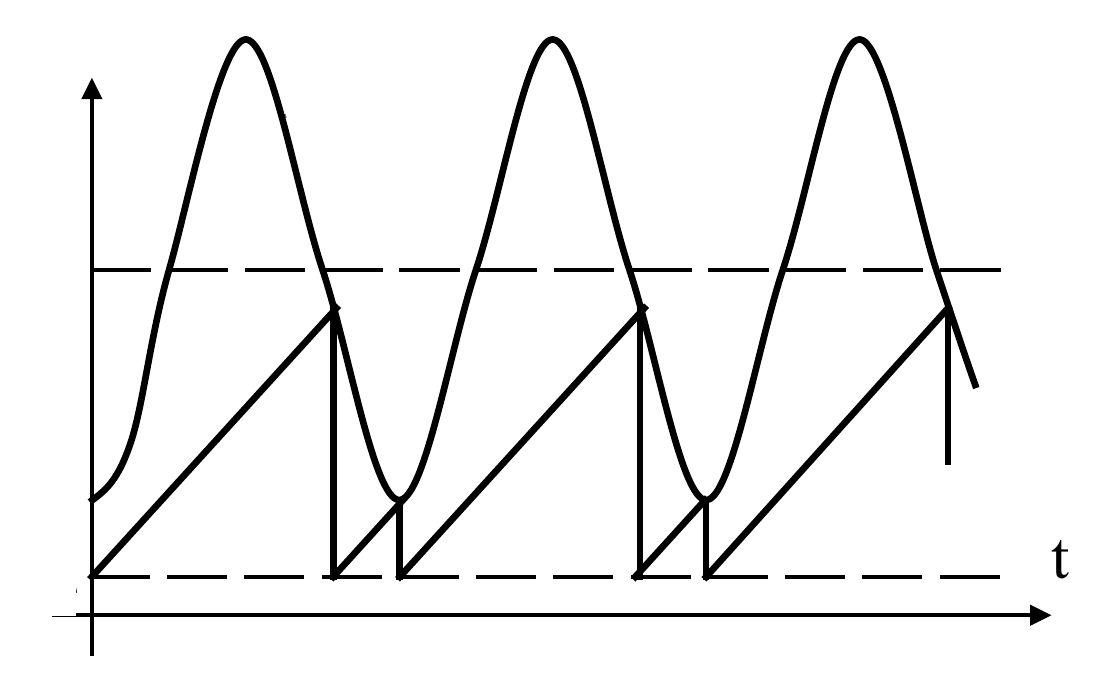
\includegraphics[width=0.8\textwidth]{fuck.png}
	\label{fig:fuck}
\end{figure}

% \newpage
% \section*{Приложение 1. Графики зависимостей} % (fold)
% \label{sec:figures}

% section figures (end)

\end{document}
